\begin{quote} \textit{2) Luego de haber estudiado como está operando el circuito con las cargas $R_1$ y $R_2$ en su valor de diseño (\SI{6}{\ohm} y\SI{1.25}{\ohm} respectivamente), estudiar cómo opera el circuito si éstas varían hacia valores mayores y menores.}
\end{quote}

	Luego, se analizó el comportamiento del circuito ante variaciones de carga, obteniéndose \ref{fig:var_R1} y \ref{fig:var_R2}. En el primer caso se varió el valor de $R_1$ en un 16\%, $R_1 \pm \SI{1}{\ohm}$, obteniéndose $\Delta V_o \simeq \SI{0.54}{\volt}$.\\
	\indent En el segundo caso se analizaron valores de $R_2$ comprendidos entre $\SI{0.5}{\ohm}$ y $\SI{2.4}{\ohm}$. No se presentan alteraciones en la tensión de salida manteniéndose constante en \SI{10.5}{\volt} aproximadamente.

\begin{figure}[H]
	\centering
	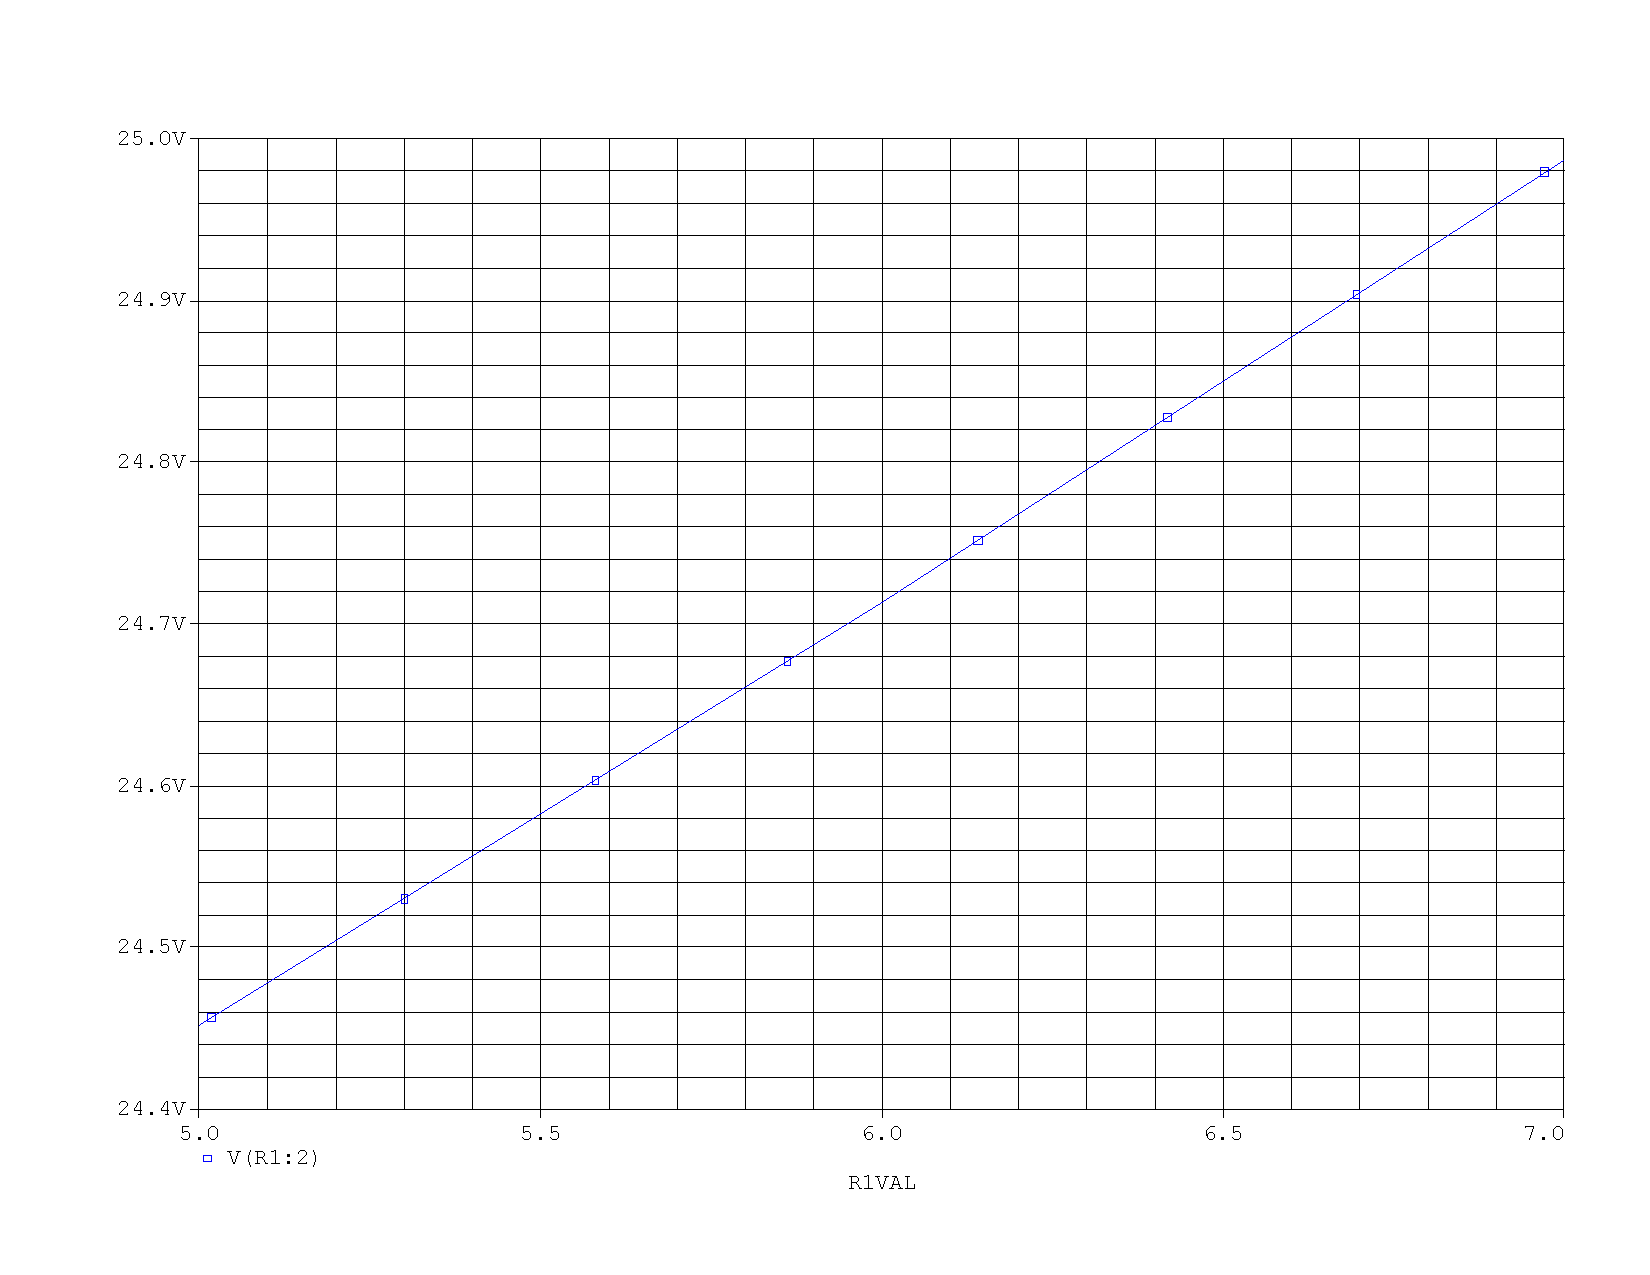
\includegraphics[scale=0.3]{Figuras/2_var_R1.pdf}
	\caption{Variación de $R_1$.}
	\label{fig:var_R1}
\end{figure}

\begin{figure}[H]
	\centering
	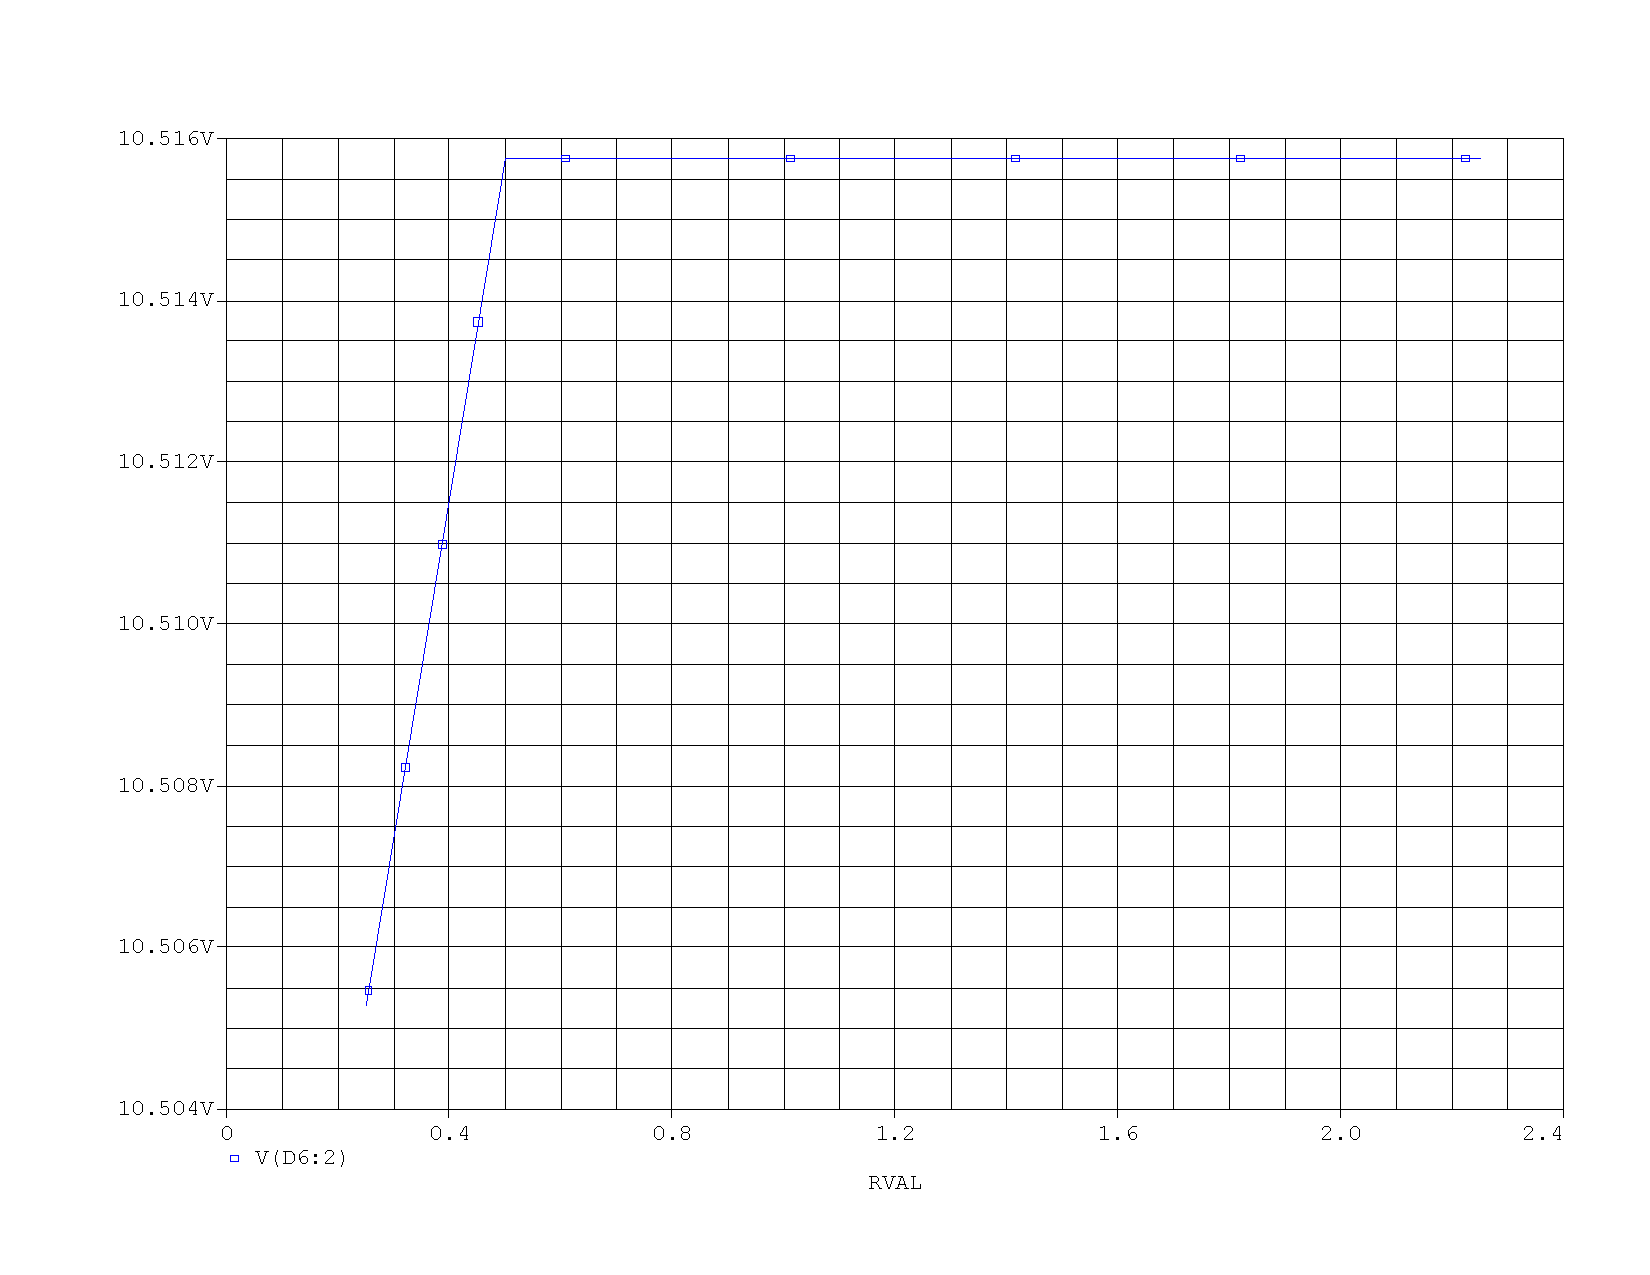
\includegraphics[scale=0.3]{Figuras/2_var_R2.pdf}
	\caption{Variación de $R_2$.}
	\label{fig:var_R2}
\end{figure}



